\documentclass[aspectratio=169]{beamer}
\usepackage[utf8]{inputenc}
\usepackage{hyperref}
\usepackage{amsmath,amsfonts,amsthm,bm}
\usepackage{color}
\usepackage{minted}
\usepackage{graphicx} % Allows including images
\usepackage{booktabs} % Allows the use of \toprule, \midrule and \bottomrule in tables
\usepackage{tikz}
\usepackage[version=3]{mhchem}
\usepackage{pgfplots}
\pgfplotsset{compat=1.16} 
\setminted{fontsize=\scriptsize}


\hypersetup{
    colorlinks=true,
    linkcolor=red,
    filecolor=magenta,      
    urlcolor=red,
}

\DeclareMathOperator*{\argmax}{argmax}
\DeclareMathOperator*{\argmin}{argmin}
\let \vec \mathbf

\newcommand{\classname}{NANOx81}
\newcommand{\classyear}{Fall 2022}
\mode<presentation> {
    \usetheme{CambridgeUS}
    \setbeamertemplate{footline}[text line]{%
      \parbox{\linewidth}{\vspace*{-8pt}\classname\hfill\classyear\hfill\insertpagenumber}}

    %\setbeamertemplate{footline}[page number]
    \setbeamertemplate{navigation symbols}{}
}


\title[Introduction to Data Science in Materials Science]{Introduction to Data Science in Materials Science}

\author{Shyue Ping Ong}
\institute[UCSD]{University of California, San Diego\\
\medskip
}
\date{\classyear} % Date, can be changed to a custom date

\begin{document}


\begin{frame}
    \titlepage % Print the title page as the first slide
\end{frame}


% \begin{frame}{Overview}
%     \tableofcontents
% \end{frame}


% \section{What is Data Science?}

\begin{frame}{What is Data Science?}
    \Huge{Data science is a multi-disciplinary field that uses scientific methods, processes, algorithms and systems to \textcolor{red}{extract knowledge and insights from structured and unstructured data}.}
\end{frame}


\begin{frame}{What is Data Science?}
    \begin{figure}
        \centering
        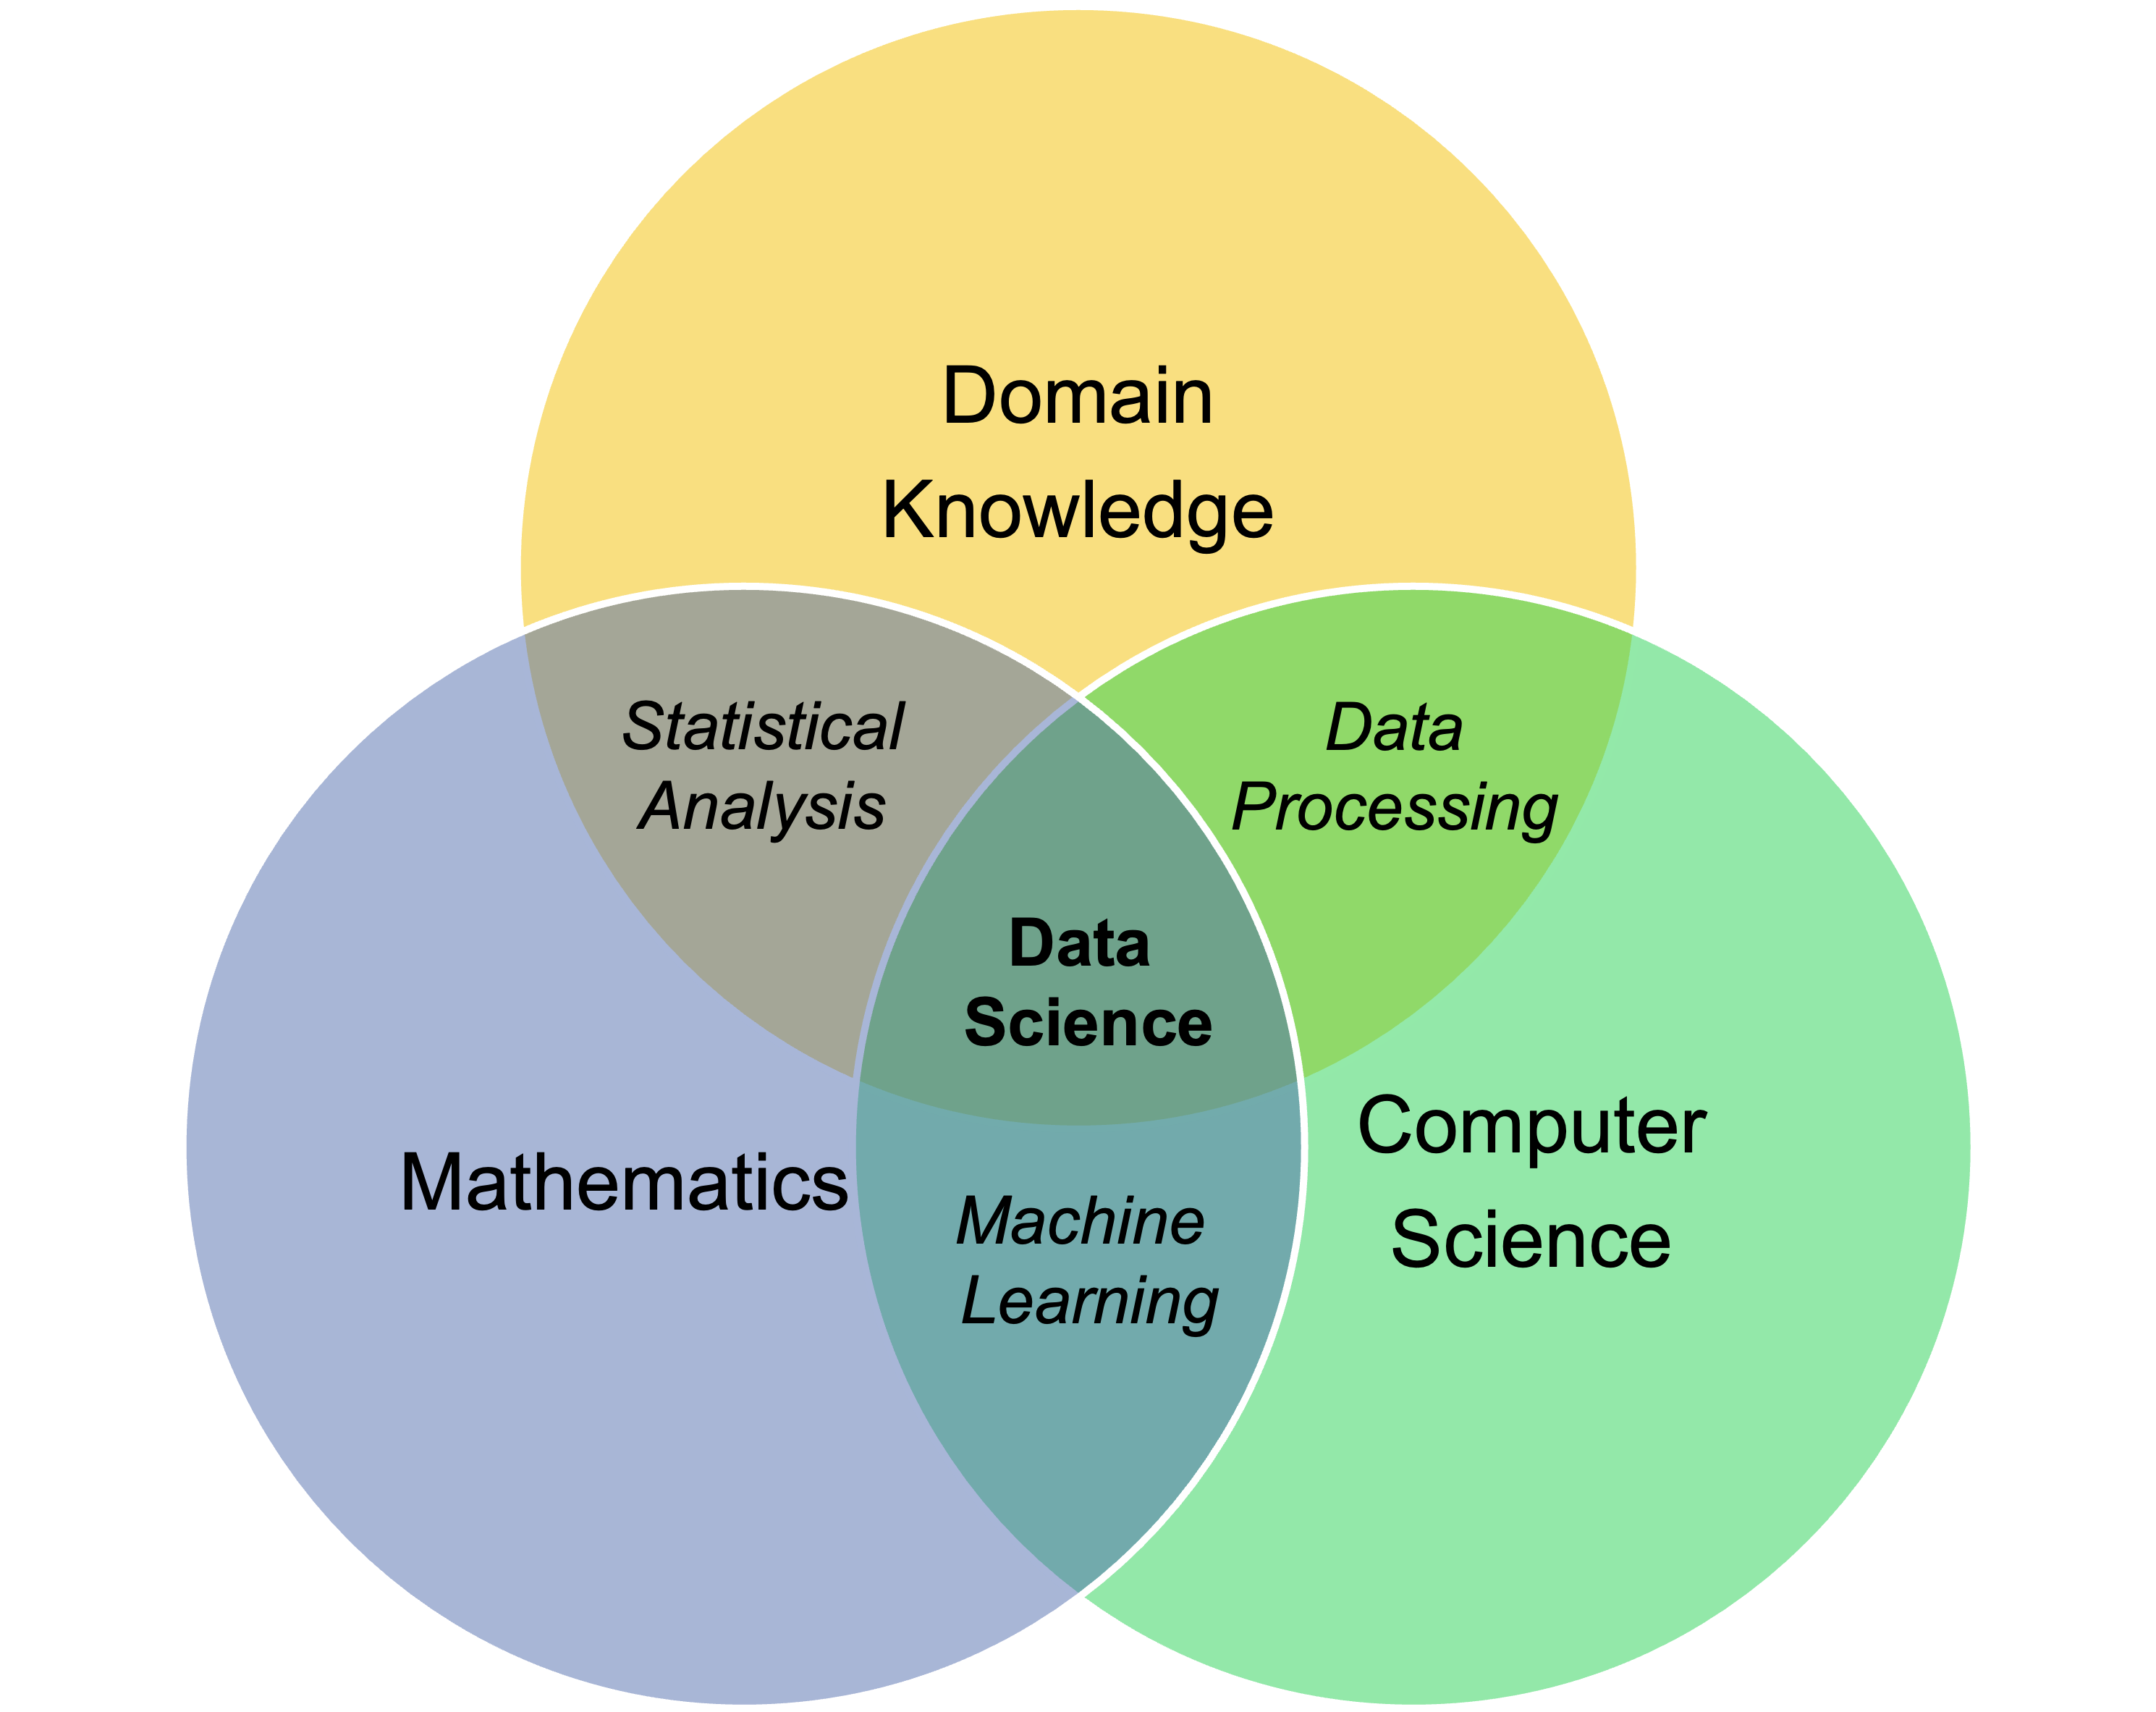
\includegraphics[width=0.5\textwidth]{lectures/slides_tex/datascience.png}    \end{figure}
\end{frame}

\begin{frame}{The Data Age}
    \begin{figure}
        \centering
        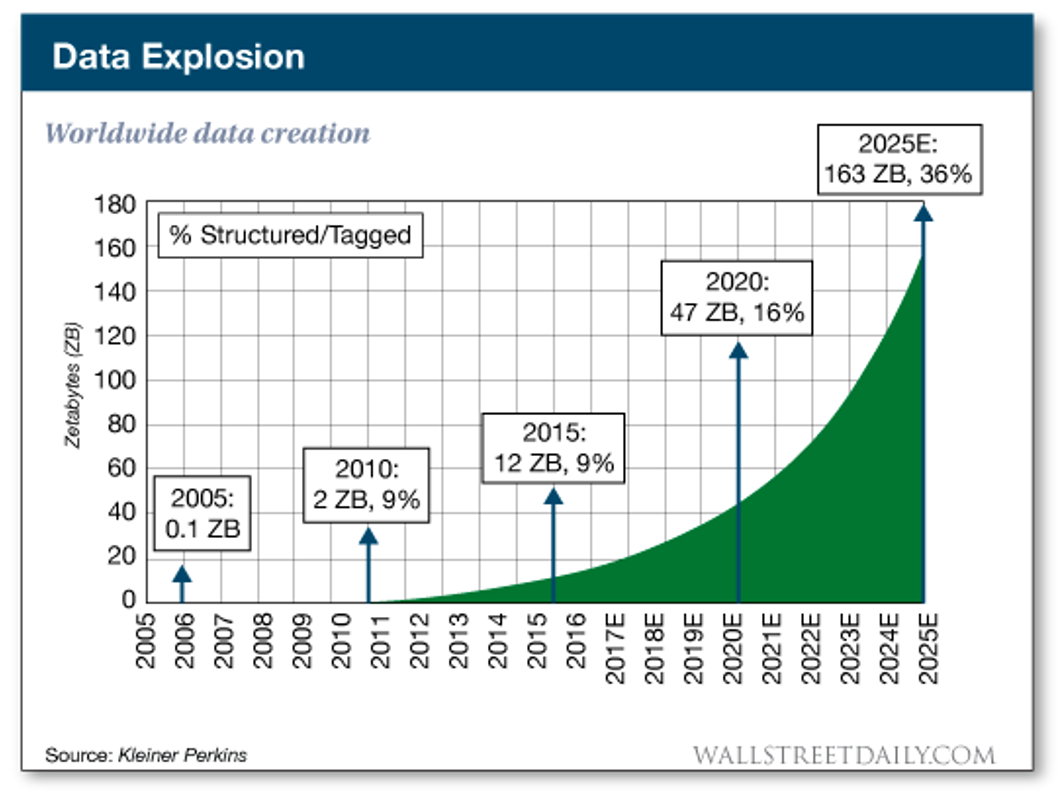
\includegraphics[width=0.6\textwidth]{lectures/slides_tex/worldwidedatacreation.png}
    \end{figure}
\end{frame}

\begin{frame}{Growth of Materials Data (as of Jan 1 2020)}

\begin{columns}
\column{0.5\textwidth}
\begin{figure}
        \centering
        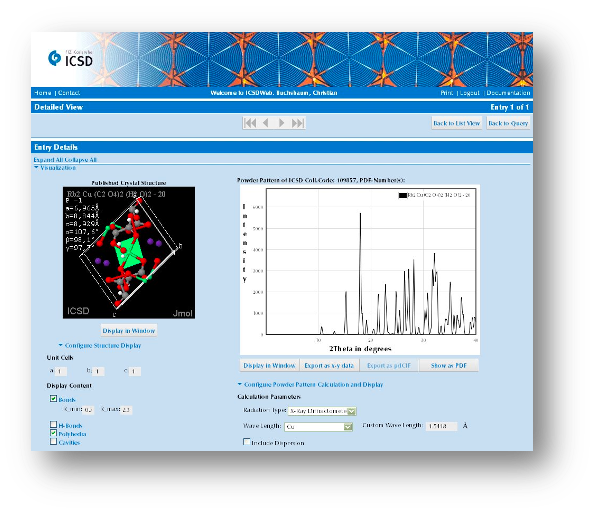
\includegraphics[width=0.4\textwidth]{lectures/slides_tex/icsd.png}
        \caption{ICSD: $sim$200,000 crystals
}
    \end{figure}
    \begin{figure}
    \centering
    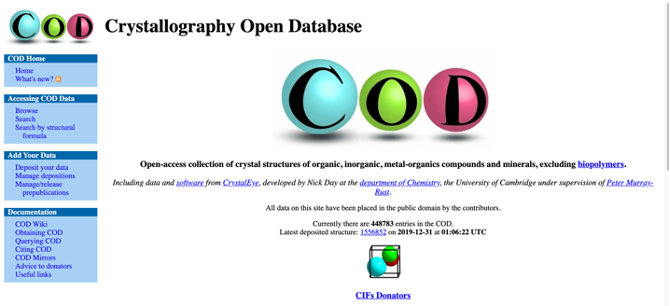
\includegraphics[width=0.4\textwidth]{lectures/slides_tex/cod.png}
    \caption{COD: $\sim$400,000 crystals
}
\end{figure}

\column{0.5\textwidth}
    \begin{figure}
        \centering
        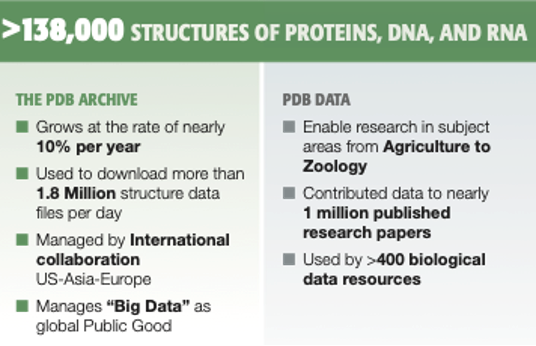
\includegraphics[width=0.4\textwidth]{lectures/slides_tex/pdb.png}
        \caption{Protein data bank}
    \end{figure}
\begin{figure}
    \centering
    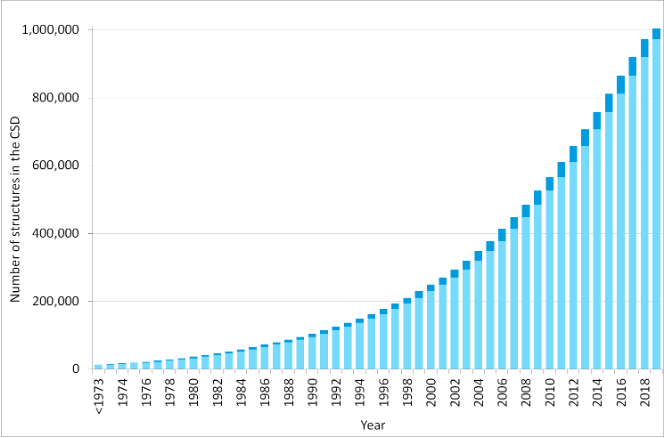
\includegraphics[width=0.4\textwidth]{lectures/slides_tex/csd.png}
    \caption{Cambridge structural database (small-molecule organic crystal structures)}
\end{figure}
\end{columns}
\end{frame}


\begin{frame}
    \Huge{\centerline{The End}}
\end{frame}

\end{document}

